\documentclass[journal,12pt,twocolumn]{IEEEtran}
\usepackage[shortlabels]{enumitem}
\usepackage{setspace}
\usepackage{gensymb}
\singlespacing
\usepackage[cmex10]{amsmath}
\usepackage{graphicx}

\usepackage{float}
\usepackage{amsthm}

\usepackage{mathrsfs}
\usepackage{txfonts}
\usepackage{stfloats}
\usepackage{bm}
\usepackage{cite}
\usepackage{cases}
\usepackage{subfig}

\usepackage{longtable}
\usepackage{multirow}

\usepackage{enumitem}
\usepackage{mathtools}
\usepackage{steinmetz}
\usepackage{tikz}
\usepackage{circuitikz}
\usepackage{verbatim}
\usepackage{tfrupee}
\usepackage[breaklinks=true]{hyperref}
\usepackage{graphicx}
\usepackage{tkz-euclide}

\usetikzlibrary{calc,math}
\usepackage{listings}
    \usepackage{color}                                            %%
    \usepackage{array}                                            %%
    \usepackage{longtable}                                        %%
    \usepackage{calc}                                             %%
    \usepackage{multirow}                                         %%
    \usepackage{hhline}                                           %%
    \usepackage{ifthen}                                           %%
    \usepackage{lscape}     
\usepackage{multicol}
\usepackage{chngcntr}

\DeclareMathOperator*{\Res}{Res}

\renewcommand\thesection{\arabic{section}}
\renewcommand\thesubsection{\thesection.\arabic{subsection}}
\renewcommand\thesubsubsection{\thesubsection.\arabic{subsubsection}}

\renewcommand\thesectiondis{\arabic{section}}
\renewcommand\thesubsectiondis{\thesectiondis.\arabic{subsection}}
\renewcommand\thesubsubsectiondis{\thesubsectiondis.\arabic{subsubsection}}


\hyphenation{op-tical net-works semi-conduc-tor}
\def\inputGnumericTable{}  %%
\newtheorem{theorem}{Theorem}[section]
\newtheorem{defn}[theorem]{Definition}
\lstset{
%language=C,
frame=single, 
breaklines=true,
columns=fullflexible
}
\begin{document}

\newcommand{\BEQA}{\begin{eqnarray}}
\newcommand{\EEQA}{\end{eqnarray}}
\newcommand{\define}{\stackrel{\triangle}{=}}
\bibliographystyle{IEEEtran}
\raggedbottom
\setlength{\parindent}{0pt}
\providecommand{\mbf}{\mathbf}
\providecommand{\pr}[1]{\ensuremath{\Pr\left(#1\right)}}
\providecommand{\qfunc}[1]{\ensuremath{Q\left(#1\right)}}
\providecommand{\sbrak}[1]{\ensuremath{{}\left[#1\right]}}
\providecommand{\lsbrak}[1]{\ensuremath{{}\left[#1\right.}}
\providecommand{\rsbrak}[1]{\ensuremath{{}\left.#1\right]}}
\providecommand{\brak}[1]{\ensuremath{\left(#1\right)}}
\providecommand{\lbrak}[1]{\ensuremath{\left(#1\right.}}
\providecommand{\rbrak}[1]{\ensuremath{\left.#1\right)}}
\providecommand{\cbrak}[1]{\ensuremath{\left\{#1\right\}}}
\providecommand{\lcbrak}[1]{\ensuremath{\left\{#1\right.}}
\providecommand{\rcbrak}[1]{\ensuremath{\left.#1\right\}}}
\theoremstyle{remark}
\newtheorem{rem}{Remark}
\newcommand{\sgn}{\mathop{\mathrm{sgn}}}
\providecommand{\abs}[1]{\vert#1\vert}
\providecommand{\res}[1]{\Res\displaylimits_{#1}} 
\providecommand{\norm}[1]{\lVert#1\rVert}
%\providecommand{\norm}[1]{\lVert#1\rVert}
\providecommand{\mtx}[1]{\mathbf{#1}}
\providecommand{\mean}[1]{E[ #1 ]}
\providecommand{\fourier}{\overset{\mathcal{F}}{ \rightleftharpoons}}
%\providecommand{\hilbert}{\overset{\mathcal{H}}{ \rightleftharpoons}}
\providecommand{\system}{\overset{\mathcal{H}}{ \longleftrightarrow}}
	%\newcommand{\solution}[2]{\textbf{Solution:}{#1}}
\newcommand{\solution}{\noindent \textbf{Solution: }}
\newcommand{\cosec}{\,\text{cosec}\,}
\providecommand{\dec}[2]{\ensuremath{\overset{#1}{\underset{#2}{\gtrless}}}}
\newcommand{\myvec}[1]{\ensuremath{\begin{pmatrix}#1\end{pmatrix}}}
\newcommand{\mydet}[1]{\ensuremath{\begin{vmatrix}#1\end{vmatrix}}}
\numberwithin{equation}{subsection}
\makeatletter
\@addtoreset{figure}{problem}
\makeatother
\let\StandardTheFigure\thefigure
\let\vec\mathbf
\renewcommand{\thefigure}{\theproblem}
\def\putbox#1#2#3{\makebox[0in][l]{\makebox[#1][l]{}\raisebox{\baselineskip}[0in][0in]{\raisebox{#2}[0in][0in]{#3}}}}
     \def\rightbox#1{\makebox[0in][r]{#1}}
     \def\centbox#1{\makebox[0in]{#1}}
     \def\topbox#1{\raisebox{-\baselineskip}[0in][0in]{#1}}
     \def\midbox#1{\raisebox{-0.5\baselineskip}[0in][0in]{#1}}
\vspace{3cm}
\title{Assignment 3}
\author{CS20BTECH11028}
\maketitle
\newpage
\bigskip
\renewcommand{\thefigure}{\theenumi}
\renewcommand{\thetable}{\theenumi}
Download all python codes from 
\begin{lstlisting}
https://github.com/Harsha24112002/AI1103/tree/main/Assignment-3/codes
\end{lstlisting}
%
and latex-tikz codes from 
%
\begin{lstlisting}
    https://github.com/Harsha24112002/AI1103/tree/main/Assignment-3
\end{lstlisting}
\section{Problem GATE MA 2012 30}
The probability density function of a random variable X is
\begin{equation}
f(x)=
\begin{cases}
\frac{1}{\lambda}e^{\brak{-\frac{x}{\lambda}}}, & x>0\\
0, & x\leq 0
\end{cases}
\end{equation}
where $\lambda>0.$ For testing the hypothesis $H_{0}:\lambda=3$ against $H_{1}:\lambda=5$, a test is given as "Reject $H_0$ if $X\geq 4.5$".The probability of type 1 error and power of the test are respectively: 
\begin{enumerate}[(A)]
\begin{multicols}{2}
\setlength\itemsep{1em}

\item 0.1353 and 0.4966\\
\item 0.1827 and 0.379\\
\item 0.2021 and 0.4493\\
\item 0.2231 and 0.4066

\end{multicols}
\end{enumerate}
\section{Solution}
\begin{defn}
\label{Type 1 error}A type 1 error occurs if the null hypothesis $H_{0}$ is rejected even if it is true.
\end{defn}
\begin{defn}
\label{Power of the test}The probability that the alternative hypothesis $H_{1}$ is true is defined to be Power of a given test. 
\end{defn}
Given,
\begin{equation}
f_{X}(x)=
\begin{cases}
\frac{1}{\lambda}e^{\brak{-\frac{x}{\lambda}}}, & x>0\\
0, & x\leq 0
\end{cases}
\end{equation}

Let cumulative distribution function be $F_{X}(x)$ for a given $\lambda$.\\
Hence,
\begin{equation}
    F_{X}(x)=\int_{-\infty}^{x}f_{X}(a) da
\end{equation}

From the probability density function,
\begin{align}
    \implies F_X(4.5)&=\int_{-\infty}^{x}f_{X}(a) da\\
    &=\int_{0}^{4.5}\frac{1}{\lambda}e^{\brak{-\frac{a}{\lambda}}}da\\
    &=1-e^{-\frac{4.5}{\lambda}}
\end{align}
We need the probability for $X\geq 4.5$,hence
\begin{align}
\text{Required probability}&=1-F_{X}(4.5)\\
&=e^{-\frac{4.5}{\lambda}}\label{eq:2.0.7}
\end{align}
Now the probability that the given null hypothesis$(H_{0})$ is true is ,\\
From \eqref{eq:2.0.7}
\begin{align}
    \text{Required probability} &=e^{-\frac{4.5}{3}}\\
    &=0.2231.
\end{align}
Therefore the probability that we are rejecting a null hypothesis which is true for $X \geq 4.5$ is 0.2231.\\
Hence the \textbf{probability of type 1 error is 0.2231}.\\
\begin{figure}[H]
    \centering
    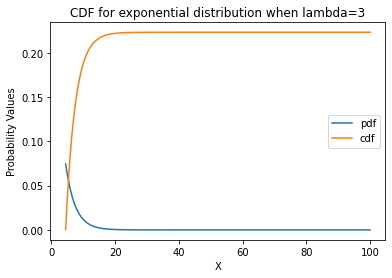
\includegraphics[scale=0.6]{1.png}
    \caption{Probability of type 1 error}
\end{figure}
Now the probability that the given alternative hypothesis($H_{1}$) is true is,\\
From \eqref{eq:2.0.7}
\begin{align}
\text{Required probability}&=e^{-\frac{4.5}{5}}\\
    &=0.4066
\end{align}
Hence the probability that the given alternative hypothesis is true for $X \geq 4.5$ is 0.4066.\\
Thus,\textbf{The power of the test is 0.4066}
\begin{figure}[H]
    \centering
    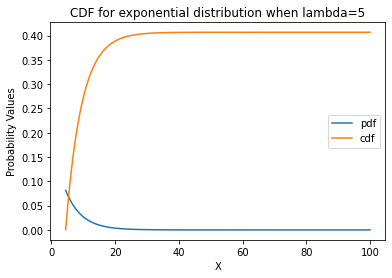
\includegraphics[scale=0.6]{2.png}
    \caption{Power of test}
\end{figure}
\end{document}